\newpage 

\section{Flow chart}
\begin{figure}
\centering
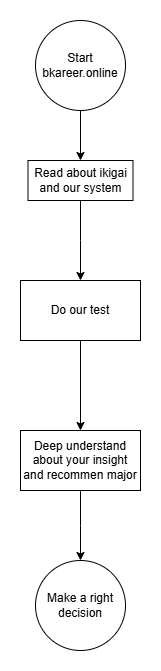
\includegraphics[width=0.8\textwidth]{images/flowchart.png}
\vspace{0.5cm}
\caption{Flow chart cho hệ thống }
\end{figure}

FlowChart này mô tả quy trình cách thức người dùng tiếp cận cũng như sử dụng hệ thống.
Từ việc truy cập vào trang web, thưc hiện loạt bài kiểm tra, nhận được đánh giá chi tiết về nhiều mặt khác nhau
trong tính cách con người từ đó hiểu biết sâu hơn. Cũng như nhận được những gợi ý về ngành nghề phù hợp với bản thân mình

\section{Activity Diagram}

\begin{figure}[H]
    \centering
    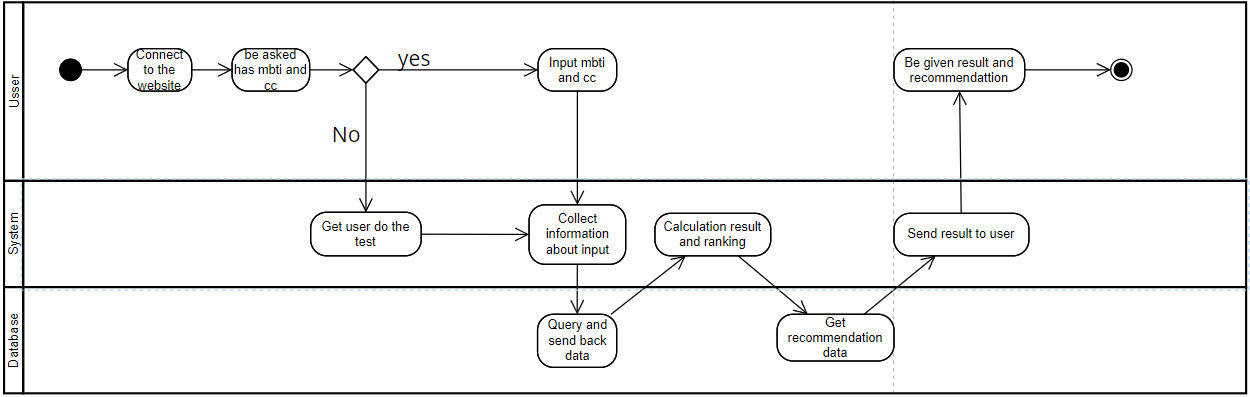
\includegraphics[width=0.8\textwidth]{images/activityDiagram.png}
    \vspace{0.5cm}
    \caption{Activity diagram cho chức năng chính của hệ thống }
\end{figure}

Activity Diagram này mô tả hoạt động của chức năng tính toán và gợi ý ngành nghề phù hợp. Sau khi người dùng truy cập vào hệ thống, họ sẽ được yêu cầu đăng nhập vào hệ thống. Sau khi chọn chức năng để tính toán kết quả gợi ý, người dùng sẽ được yêu cầu nhập kết quả của các bài kiểm tra, bao gồm bài kiểm tra tính cách MBTI, và nhóm ngành nghề phù hợp Career Clustering. Nếu như thiếu kết quả của một trong hai hoặc cả hai bài kiểm tra, người dùng sẽ được yêu cầu làm bài kiểm tra tương ứng trước, sau đó mới được chuyển hướng về lại trang gợi ý ngành nghề. Người dùng sau đó sẽ chọn một trong hai giải thuật MCDM: Weighted-sum hoặc VIKOR. Sau khi hệ thống đã nhận đầy đủ đầu vào từ người dùng (tức kết quả của hai bài kiểm tra và giải thuật người dùng lựa chọn) sẽ truy vấn đến cơ sở dữ liệu rồi trả dữ liệu về lại cho hệ thống. Hệ thống sẽ sử dụng dữ liệu và gọi các hàm tính toán để tìm ra ngành nghề phù hợp. Dữ liệu về ngành nghề phù hợp sẽ được truy vấn ngược lại cơ sở dữ liệu để đưa ra gợi ý và mô tả về nghề nghiệp. Hệ thống sau đó nhận dữ liệu về gợi ý từ cơ sở dữ liệu và in kết quả ra màn hình cho người dùng.
